\section{Aufgaben}
\newpage
\subsection{Liegestütze - Leichte Aufgabe}
\vfill
\begin{center}
    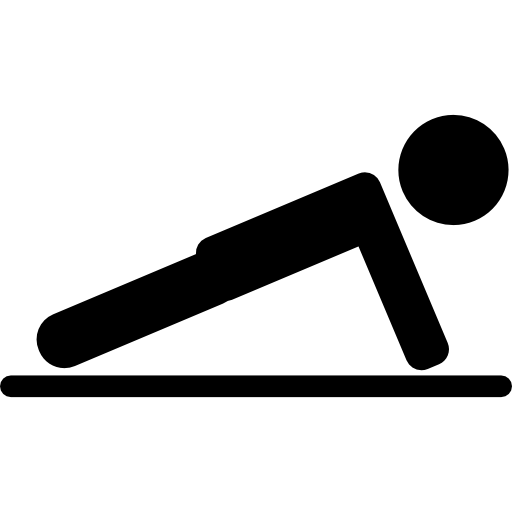
\includegraphics[height=5cm]{graphics/push_up.png}
\end{center}
\vfill
\textbf{Mache fünf Liegestütze} auf einer Isomatte.
Wenn keine Isomatte vorhanden ist, kannst du die Liegestütze auf dem Boden
ausführen.
Wer keine klassischen Liegestütze ausführen kann, kann auf leichtere
Variationen, wie Liegestütze auf den Knien, ausweichen.
\newpage

\subsection{Squats - Leichte Aufgabe}
\vfill
\begin{center}
    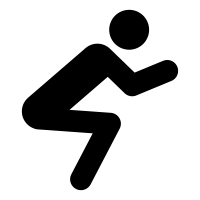
\includegraphics[height=5cm]{graphics/squat.png}
    \end{center}
\vfill
\textbf{Mache acht Squats}.
\newline
\newpage

\subsection{Tischtennisball - Leichte Aufgabe}
\vfill
\begin{center}
    
\includegraphics[height=5cm]{graphics/table_tennis.png}
\end{center}
\vfill
Nimm den Schläger in eine Hand und werfe den Ball in die Luft.
\textbf{Spiele} danach den Tischtennisball
mit dem Schläger \textbf{zehn Mal hintereinander nach oben}, ohne dass er dabei
auf den Boden fällt.
Wenn der Ball vor der zehnten Berührung auf den Boden fällt, starte die Aufgabe
neu.
Lege den Schläger nach der Aufgabe vorsichtig auf den Ball, sodass dieser nicht
wegrollt.
\newline
\newpage

\subsection{Pyramide aus Bechern - Leichte Aufgabe}
\vfill
\begin{center}
    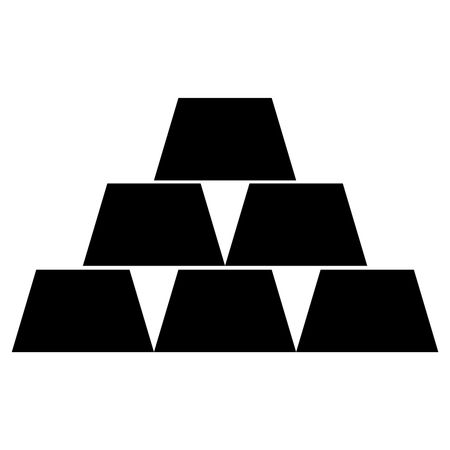
\includegraphics[height=5cm]{graphics/cup_pyramid.jpg}
\end{center}
\vfill
\textbf{Baue} eine \textbf{dreistöckige Pyramide} aus Bechern.
Baue nach der Aufgabe deine Pyramide wieder ab und staple alle Becher in einem
Stapel.
\newline
\newpage

\subsection{Eimerwurf - Leichte Aufgabe}
\vfill
\begin{center}
    
\includegraphics[height=5cm]{graphics/basketball.png}
\end{center}
\vfill
Nehme den Ball aus dem Eimer und gehe hinter die Wurflinie.
\textbf{Werfe} von dort aus den \textbf{Ball in den Eimer}.
Wenn du verfehlst, wiederhole die Aufgabe so lange, bist du triffst.
Lasse den Ball nach dem Treffer im Eimer liegen.
\newline
\newpage

\subsection{Kreuz-Ass finden - Leichte Aufgabe}
\vfill
\begin{center}
    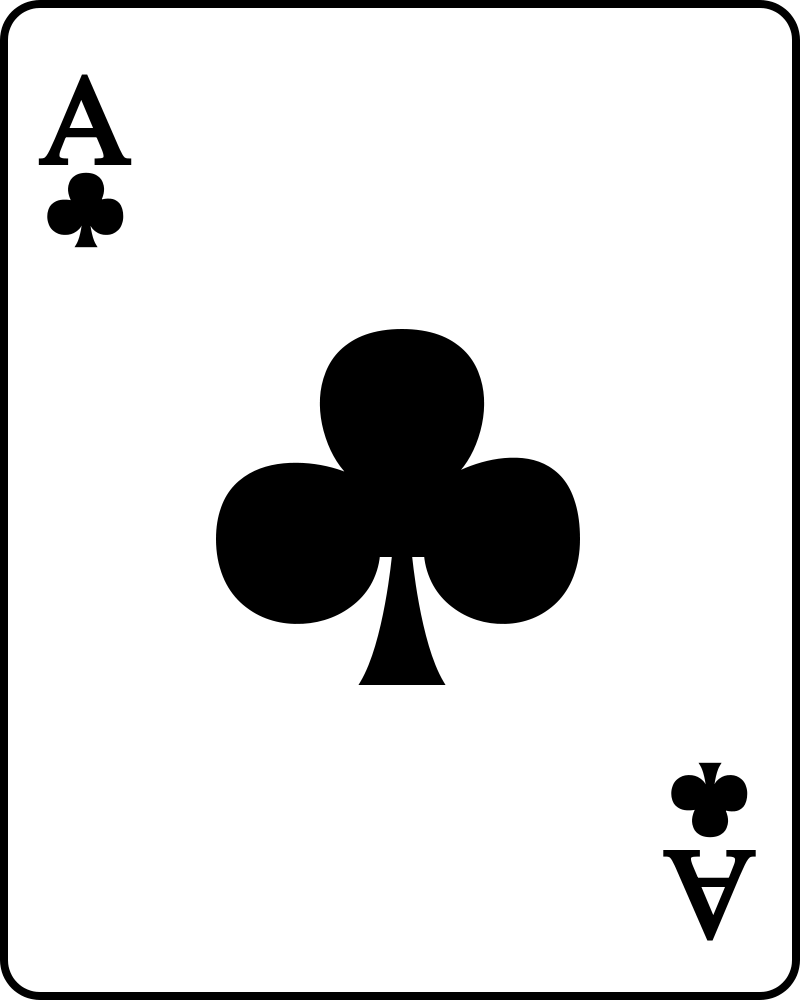
\includegraphics[height=5cm]{graphics/cross_ace.png}
\end{center}
\vfill
\textbf{Finde das Kreuz-Ass} im Skatdeck.
Wenn du das Kreuz-Ass gefunden hast, mische das Deck und lege es verdeckt
zurück.
\newline
\newpage

\subsection{Dr. Bibber - Leichte Aufgabe}
\vfill
\begin{center}
    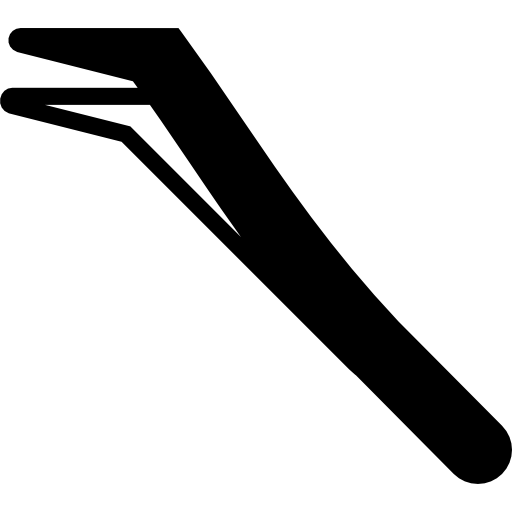
\includegraphics[height=5cm]{graphics/tweezers.png}
\end{center}
\vfill
\textbf{Entleere} den Körper von Dr. Bibber \textbf{ohne} ihn dabei
\textbf{zu berühren}.
Wenn du ihn berührst, lege alle Teile wieder in Dr. Bibber und starte neu.
Lege anschließend wieder alle Teile in Dr. Bibber.
\newline
\newpage

\subsection{Hamster-Singen - Leichte Aufgabe}
\vfill
\begin{center}
    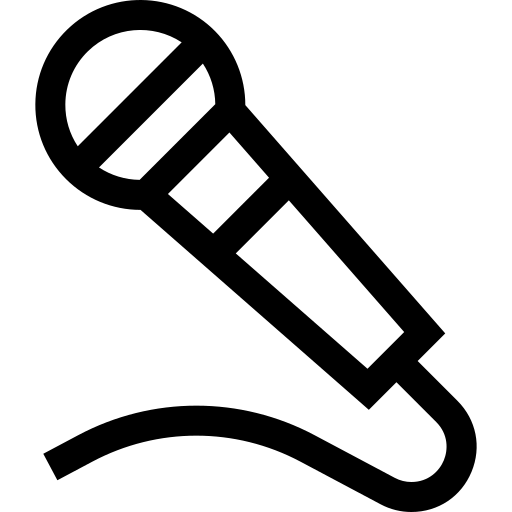
\includegraphics[height=5cm]{graphics/microfone.png}
\end{center}
\vfill
Nehme den obersten Text vom Stapel.
Stelle sicher, dass der Hamster angeschaltet ist.
\textbf{Singe} den Text, Strophe für Strophe, zusammen \textbf{mit dem Hamster}.
Lege den Text anschließend unter den Stapel.
\newline
\newpage

\subsection{Wäsche machen - Mittlere Aufgabe}
\vfill
\begin{center}
    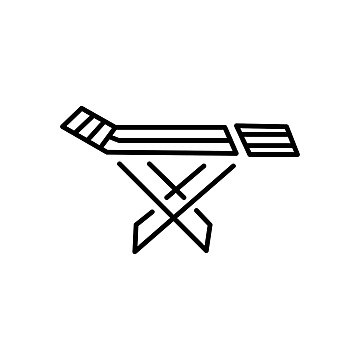
\includegraphics[height=5cm]{graphics/clothes_horse.jpg}
\end{center}
\vfill
Wenn gerade jemand die Aufgabe Wäsche machen absolviert, warte bis die Aufgabe
abgeschlossen wurde.
Gehe zu einem der beiden Wäscheständer mit Kleidung.
Wenn sich an dem aktuellen Wäscheständer keine Kleidung befindet, gehe zum
anderen Wäscheständer.
\textbf{Hänge die Kleidung ab} und packe sie in den Wäschekorb.
\textbf{Gehe} anschließend \textbf{zum anderen Wäscheständer}.
\textbf{Hänge dort} die Kleidung \textbf{wieder auf}.
Stelle den Wäschekorb vor dem Wäschekorb ab.
\newline
\newpage

\subsection{Geldtransport - Mittlere Aufgabe}
\vfill
\begin{center}
    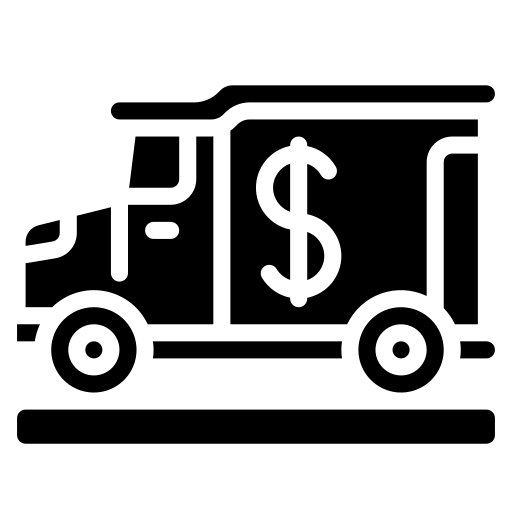
\includegraphics[height=5cm]{graphics/money_transport.png}
\end{center}
\vfill
Gehe zu einem der Geldstapel.
Befindet sich an dem Geldstapel nicht genug Geld, gehe zum anderen Geldstapel.
\textbf{Nehme} dir \textbf{420 Monopoly-Dollar} und \textbf{transportiere sie
zum anderen Geldstapel}.
Lege das Geld dort wieder unter den Stein, damit es nicht wegfliegt.
\newline
\newpage

\subsection{Eierlauf - Mittlere Aufgabe}
\vfill
\begin{center}
    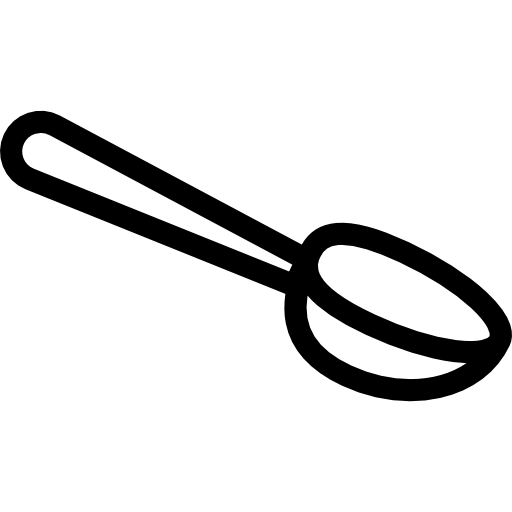
\includegraphics[height=5cm]{graphics/spoon.png}
\end{center}
\vfill
\textbf{Nehme in eine Hand einen Teelöffel und lege darauf den Ball}
ab.
\textbf{Verschränke die andere Hand hinter deinem Rücken} und behalte sie dort.
\textbf{Laufe} mit dem Ball auf dem Teelöffel \textbf{bis zur Markierung und
zurück, ohne dass
der Ball dabei auf den Boden fällt}. Falls der Ball auf der Strecke auf den Boden
fällt, starte neu.
Lege den Ball und Löffel nach der Aufgabe so hin, sodass der Ball nicht
wegrollt.
\newline
\newpage

\subsection{Mini Sudoku}
\vfill
\begin{center}
    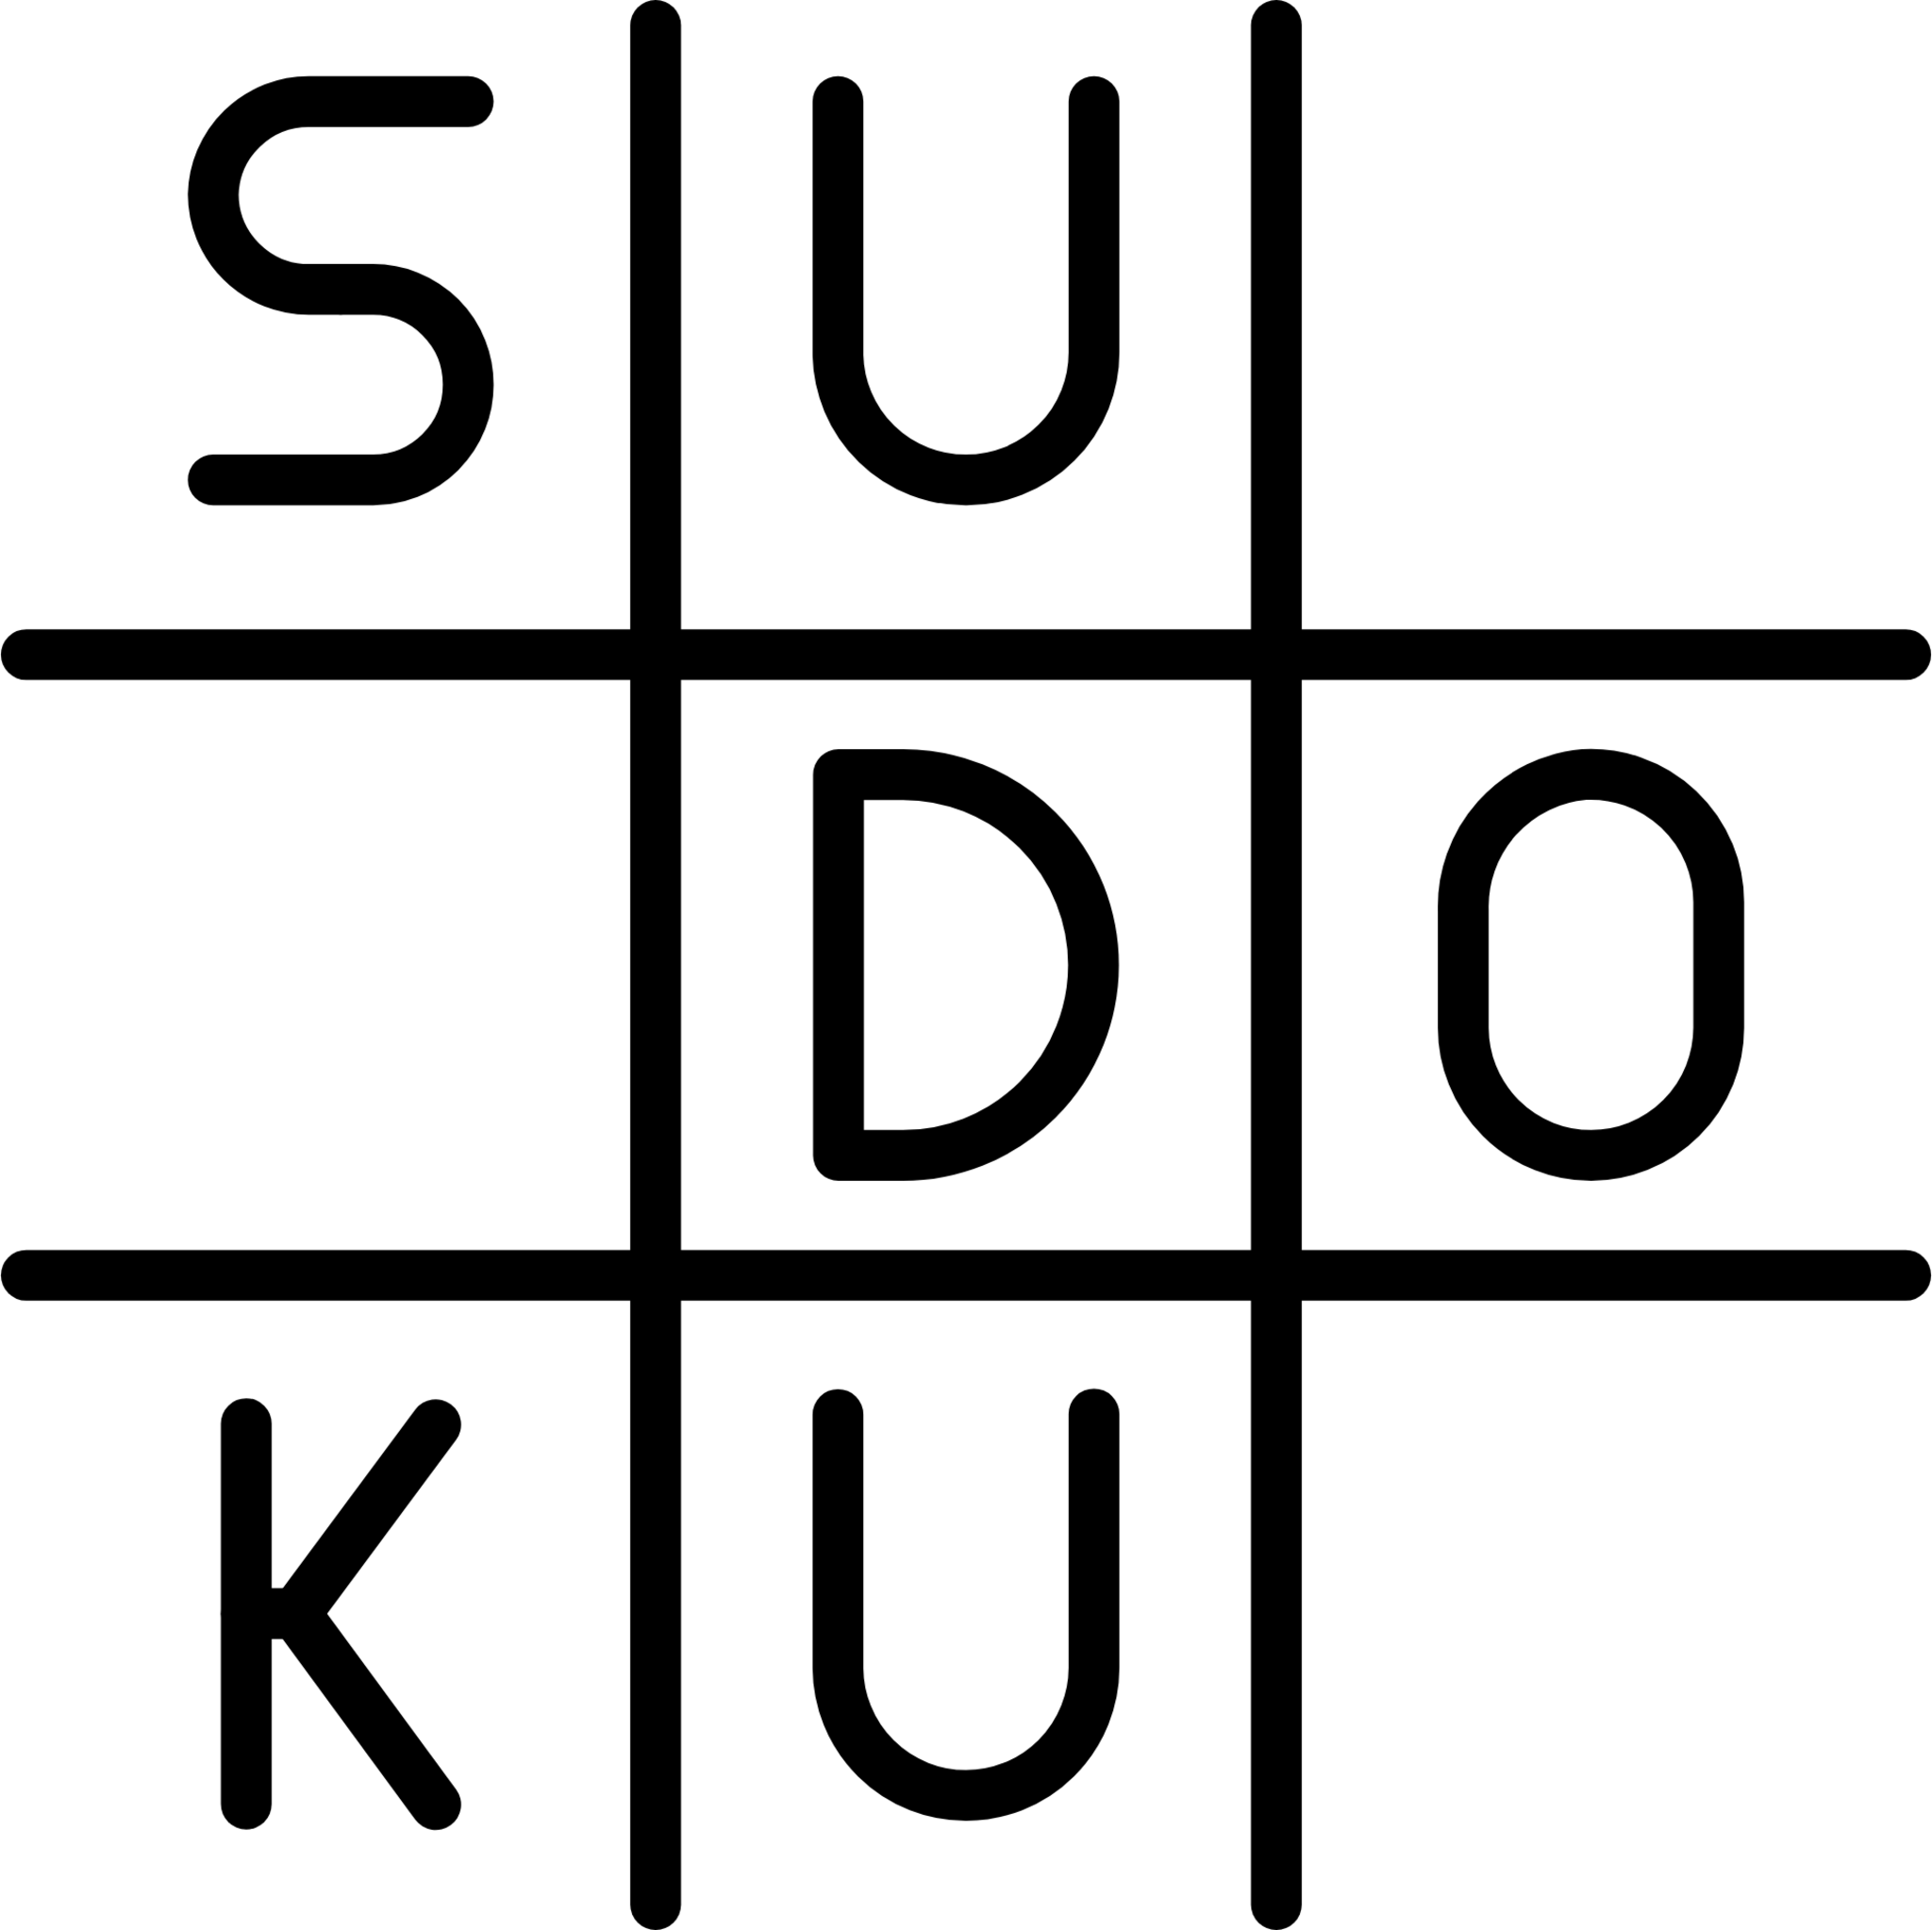
\includegraphics[height=5cm]{graphics/sudoku.png}
\end{center}
\vfill
Nehme den Stift und das oberste Mini Sudoku vom Stapel.
\textbf{Löse das Mini Sudoku}.
Lege anschließend das Sudoku unter den Stapel und den Stift auf den Stapel,
sodass dieser nicht wegfliegt.
\newline
\newpage
